\chapter{Redes Neuronales Convolucionales}\label{cap:red_neuronal_convolucional}

A raíz de las limitaciones encontradas en las redes neuronales tradicionales, el mundo de la visión por computador se vio "forzado" a buscar otras técnicas más especializadas. No sólo desde el punto de vista de la precisión de los modelos, sino también, del rendimiento. Como hemos comentado en secciones anteriores, los modelos de inferencia tradicional necesitan una gran cantidad de recursos para poder trabajar con información espacial, factor que en muchas ocasiones se convierte en limitante.

La necesidad de un enfoque más eficiente dio lugar al desarrollo de las Redes Neuronales Convolucionales, que basan su funcionamiento en la operación de la convolución. Esta herramienta matemática permite extraer características de conjuntos de datos $n$-dimensionales guardando las relaciones espaciales entre los nodos, lo que la convierte en la candidata perfecta para superar las limitaciones presentadas por arquitecturas tradicionales. Estas técnicas permiten a los modelos de convolución \textbf{reconocer patrones locales} y elementos como bordes, texturas o contornos y sus relaciones entre diferentes regiones de una imagen de una forma más natural, como hacemos los seres humanos para reconocer objetos como pelotas, coches, animales, etc.

\begin{figure}[ht]
	\centering
	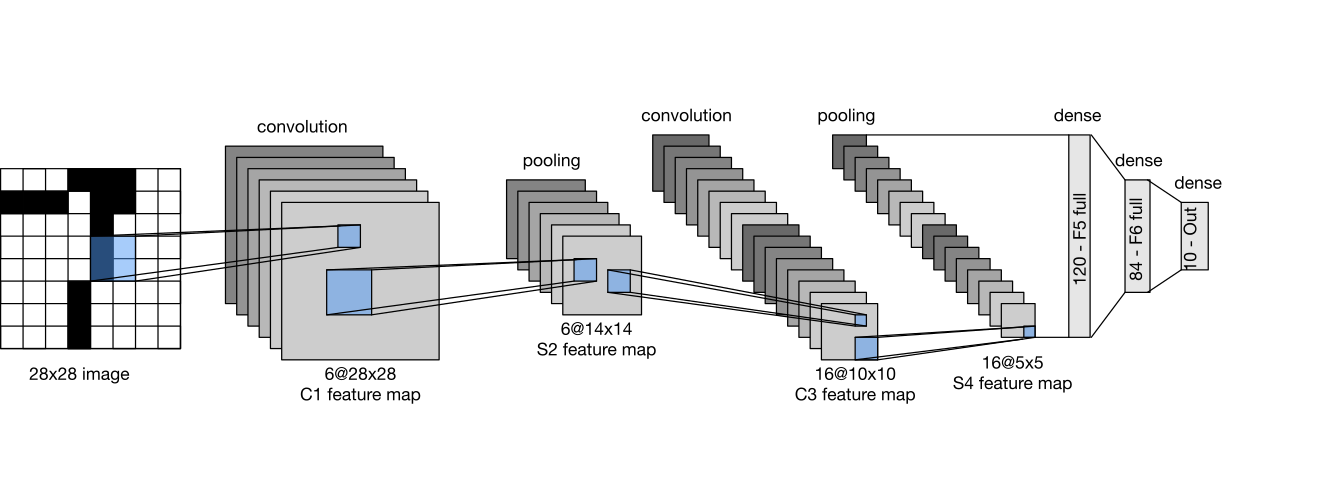
\includegraphics[width=1\linewidth]{figures/ejemplos/LeNet-5_architecture.png}
	\caption{Arquitectura LeNet-5 \cite{zhang2023dive}.}
	\label{img:lenet-5}
\end{figure}

Por otro lado, la arquitectura convolucional nos permite simplificar mucho la cantidad de parámetros que debe gestionar el modelo para llevar a cabo su tarea, en comparación con modelos tradicionales, como los perceptrones multicapa (MLP, en inglés), donde fácilmente podemos llegar a acumular centenas de miles de parámetros de conexiones entre cada par de neuronas. Esto es gracias a la \textbf{compartición de pesos} en las capas de convolución, que utilizan filtros (cuyos valores son parámetros de la red) que se aplican repetidamente sobre diferentes regiones de la imagen, lo que nos permite, no sólo encontrar patrones similares en diferentes regiones, sino que también reducir drásticamente el consumo de memoria, mejorar la eficiencia y la generalización del modelo.

Otro aspecto fundamental de las redes convolucionales es su capacidad para realizar una \textbf{descomposición jerárquica} de las características presentes en los datos de entrada. En las capas iniciales, los filtros tienden a detectar patrones muy simples, como bordes horizontales, verticales o diagonales. Conforme se avanza en profundidad, las siguientes capas combinan estas representaciones elementales para formar descriptores más complejos, como esquinas, texturas o regiones específicas de un objeto. Finalmente, en las capas más profundas, la red es capaz de representar estructuras de alto nivel a partir de la composición de las características aprendidas previamente. Este proceso refleja, en cierto modo, la manera en que el sistema visual humano descompone la información visual en niveles de complejidad creciente \cite{dl_python__chollet_2021, nn_dl__michael_nielsen_2015, dl__goodfellow_2016}.

Algunos de los hitos más relevantes en modelos convolucionales fueron la arquitectura \textit{LeNet-5}, propuesta por \citeauthor{lecun-98} en \citeyear{lecun-98}, diseñada para el reconocimiento de dígitos y letras manuscritas. Este modelo mostró por primera vez el potencial de las convoluciones para extraer características jerárquicas de las imágenes de forma automática, tanto que esta tecnología acabó implementándose en las máquinas bancarias ATM para leer cheques \cite{lecun-98}.

\begin{figure}[ht]
	\centering
	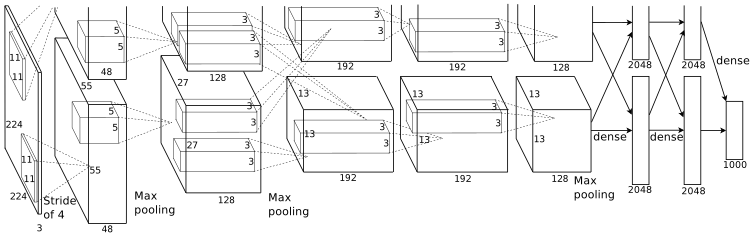
\includegraphics[width=1\linewidth]{figures/ejemplos/AlexNet_Original_block_diagram.png}
	\caption{Arquitectura AlexNet \cite{Krizhevsky2012ImageNetCW}.}
	\label{img:alexnet}
\end{figure}


Más tarde, por el año 2012, el interés en las redes convolucionales incrementó cuando \textit{AlexNet}, un modelo de clasificación convolucional logró una mejora drástica en el ILSVRC (\textit{ImageNet Large Scale Visual Recognition Challenge}), una competición mundialmente conocida por evaluar el rendimiento y desempeño de arquitecturas de detección de objetos y clasificación de imágenes de gran tamaño \cite{imagenet-web}. Este novedoso modelo consiguió reducir a la mitad el error de clasificación respecto al mejor sistema hasta ese momento \cite{Krizhevsky2012ImageNetCW}. Este resultado marcó el inicio de la adopción masiva de los modelos convolucionales y consolidó su papel como modelo de referencia en visión por computador.

Actualmente, las redes convolucionales tienen una amplia variedad de aplicaciones prácticas: reconocimiento facial en sistemas de seguridad, detección de objetos en conducción autónoma, análisis médico de imágenes como radiografías o resonancias magnéticas, clasificación de imágenes por satélite o incluso el procesamiento de vídeo en tiempo real \cite{nn_fundamentals__thakur_2021, rna_fundamentos__hilera_2021, conv_nn_face_recog__chowanda_2019}.



\section{Arquitectura de una Red Neuronal Convolucional}\label{sec:arquitectura_cnn}

Las redes convolucionales son famosas por su arquitectura que, a menudo, recuerda a la forma de un embudo. Se desglosa en una serie de capas con orden concreto. Cada una de ellas está especializada en tareas concretas para obtener cierta información de las entradas. Esta configuración permite a la red aprender representaciones progresivamente más abstractas y complejas.


\paragraph{Capa convolucional}

Además de darle el nombre a la arquitectura, es en esta capa en la que reside la clave del éxito de los modelos convolucionales. Como mencionamos anteriormente, la principal diferencia con los modelos tradicionales se encontraba en la forma en la que se interpreta y relaciona la información espacial de los datos de entrada a la red. Esto es posible gracias a la operación de convolución que llevan a cabo en su interior.

La \textbf{convolución} es un operador matemático que transforma dos funciones $f$ y $g$ en una tercera función que, de cierta forma, representa la superposición de $f$ y $g$ a lo largo del tiempo \cite{dl__goodfellow_2016}. Intuitivamente, puede entenderse como una operación en la que una de las funciones se "desliza" sobre la otra, midiendo en cada posición el grado de similitud entre ambas.

\begin{figure}[ht]
	\centering
	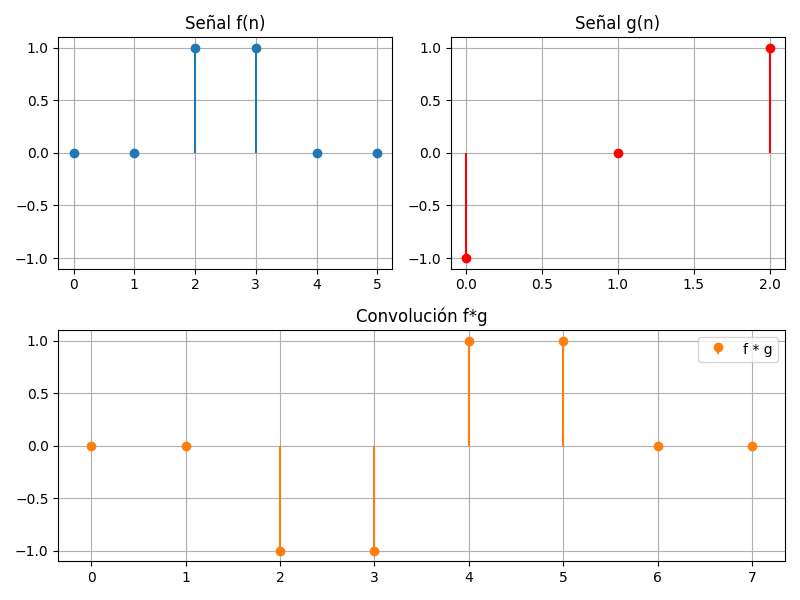
\includegraphics[width=0.7\linewidth]{figures/ejemplos/convolucion_f_g_discretas.png}
	\caption{Convolución discreta entre $f = [0,0,1,1,0,0]$ y filtro de detección de bordes $g = [-1,0,1]$.}
	\label{fig:convolucion_f_g_discreta}
\end{figure}

En las capas convolucionales, consiste en desplazar pequeñas matrices denominanadas \textit{filtros} o \textit{kernels} a lo largo de la imagen de entrada a la capa y realizar una serie de cálculos entre los valores de nuestra matriz y los de la entrada que nos ayudarán a detectar características importantes \cite{nn_dl__michael_nielsen_2015}.

\begin{figure}[ht]
	\centering
	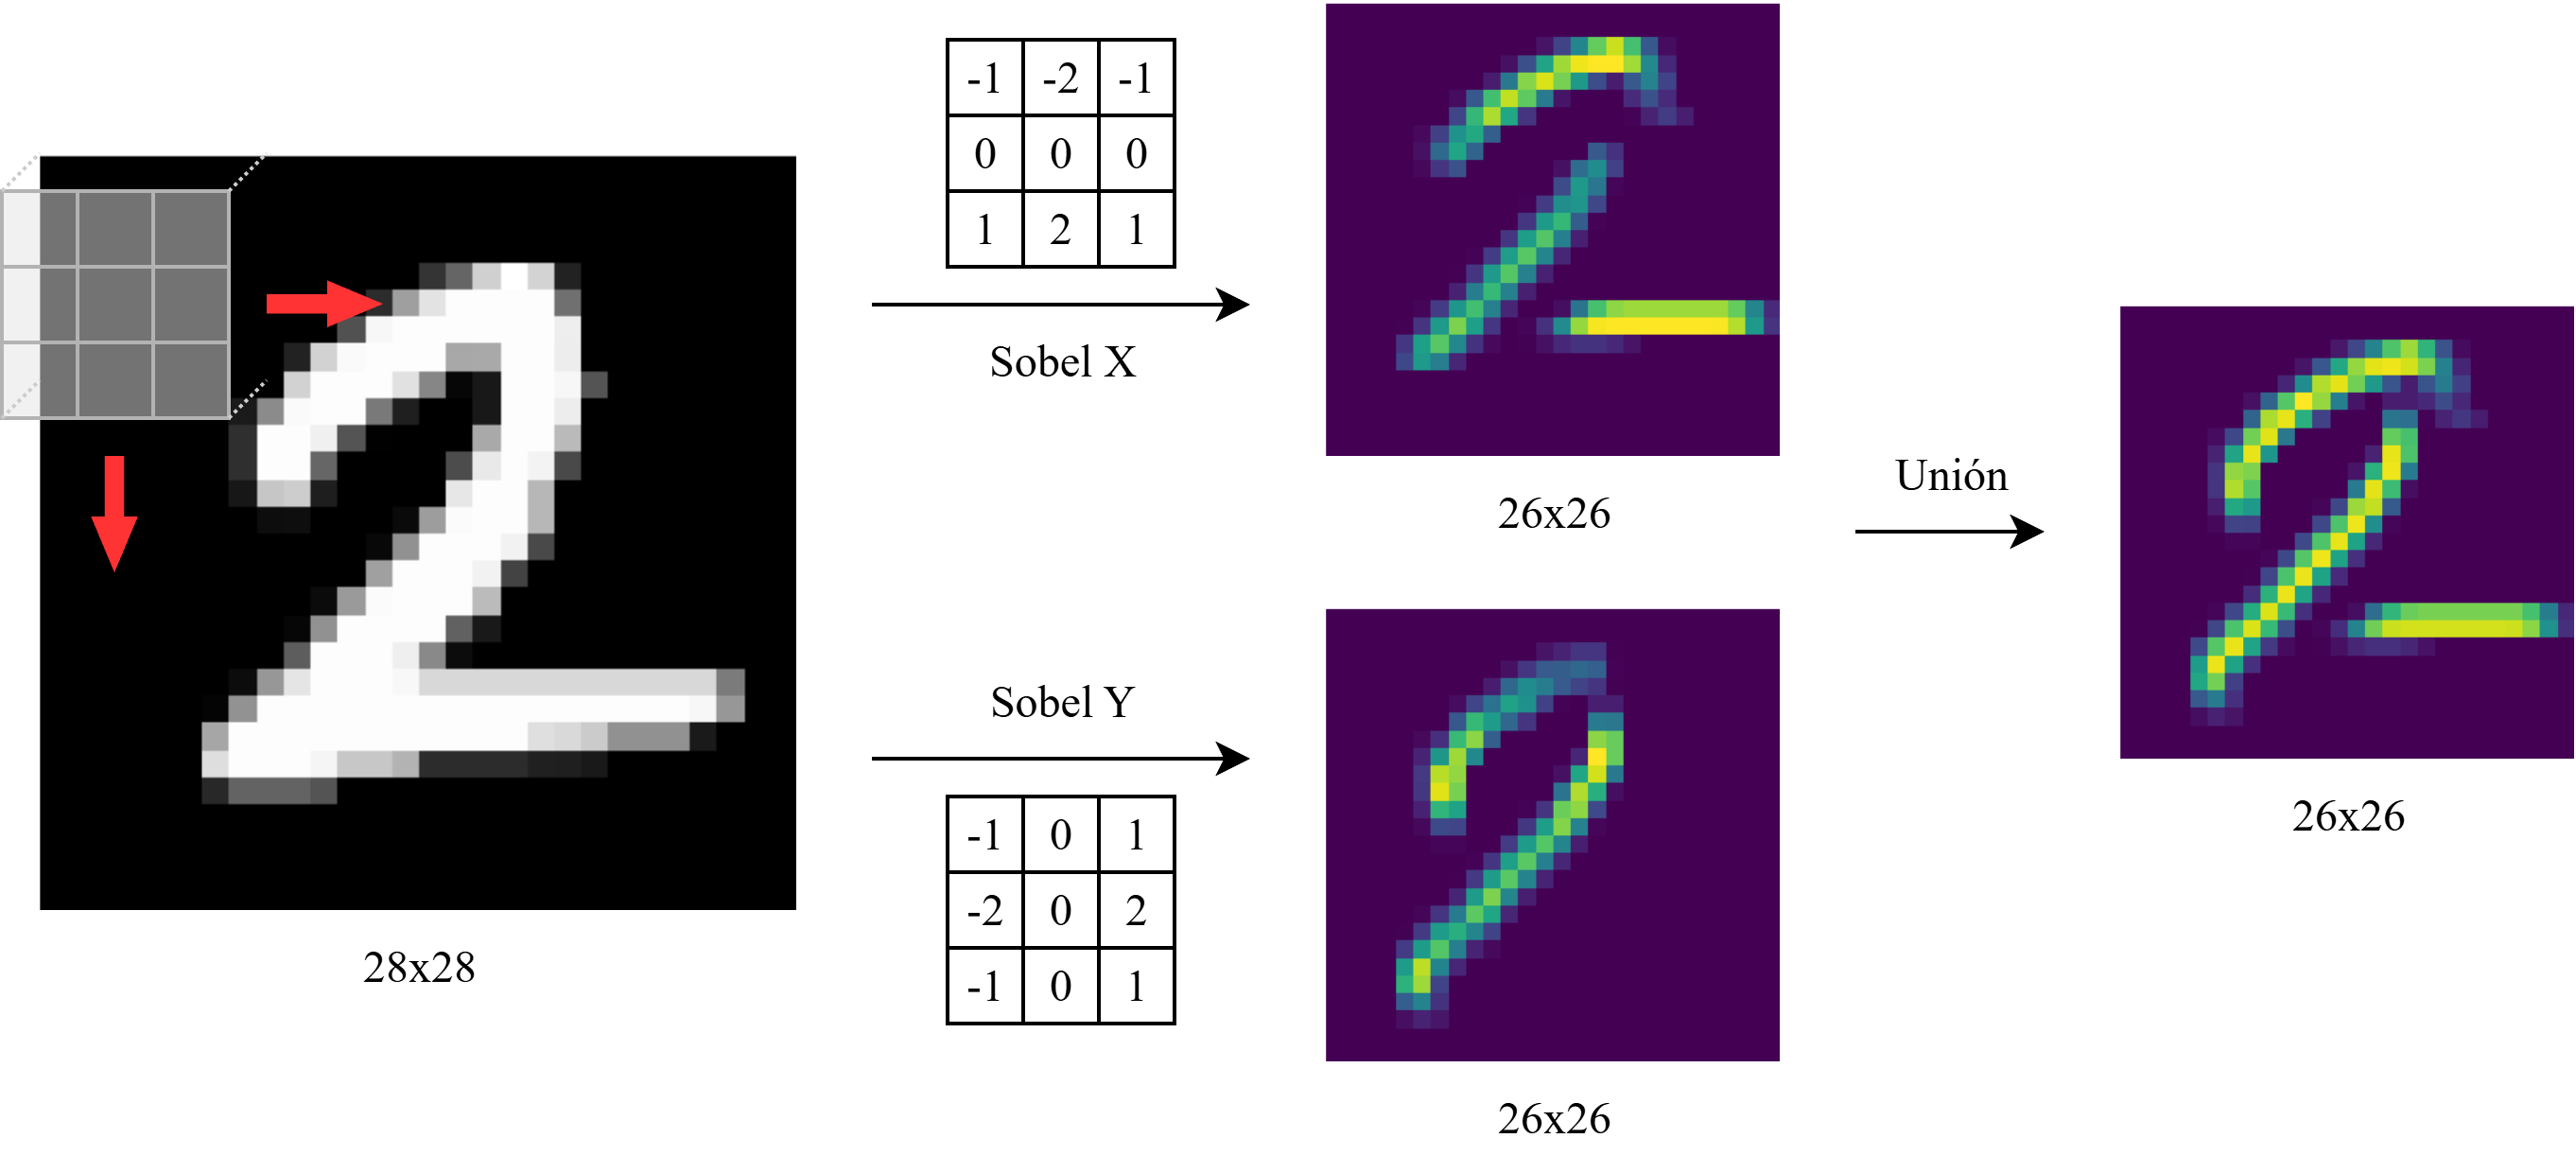
\includegraphics[width=1\linewidth]{figures/ejemplos/convolucion_sobel.png}
	\caption{Convolución con filtro de Sobel en ejes ${x,y}$ para detectar bordes.}
	\label{fig:convolucion_sobel}
\end{figure}

Por ejemplo, en la figura \ref{fig:convolucion_sobel}, hemos aplicado el filtro de Sobel, kernel conocido por su capacidad para localizar bordes verticales y horizontales, para localizar las regiones de la imagen en las que podemos encontrar dichas características. Cada una de estas detecciones puede ser una de las salidas de un filtro de las primeras capas de convolución de la red. A medida que avanza la información por las diferentes capas convolucionales, se irán detectando más características, consiguiendo que la red sea capaz de captar detalles más concretos, como curvas, o contornos. Claro que, a diferencia de este ejemplo, en una capa convolucional generalmente obtenemos muchas más salidas, concretamente, tantas como filtros pasemos, por ejemplo, la salida de pasar una imagen de $28\times28$ por una capa convolucional con 32 filtros de $3\times3$ nos devuelve $32$ imágenes de $26\times26$ (fig. \ref{fig:conv1_salidas}).

\begin{figure}[ht]
	\centering
	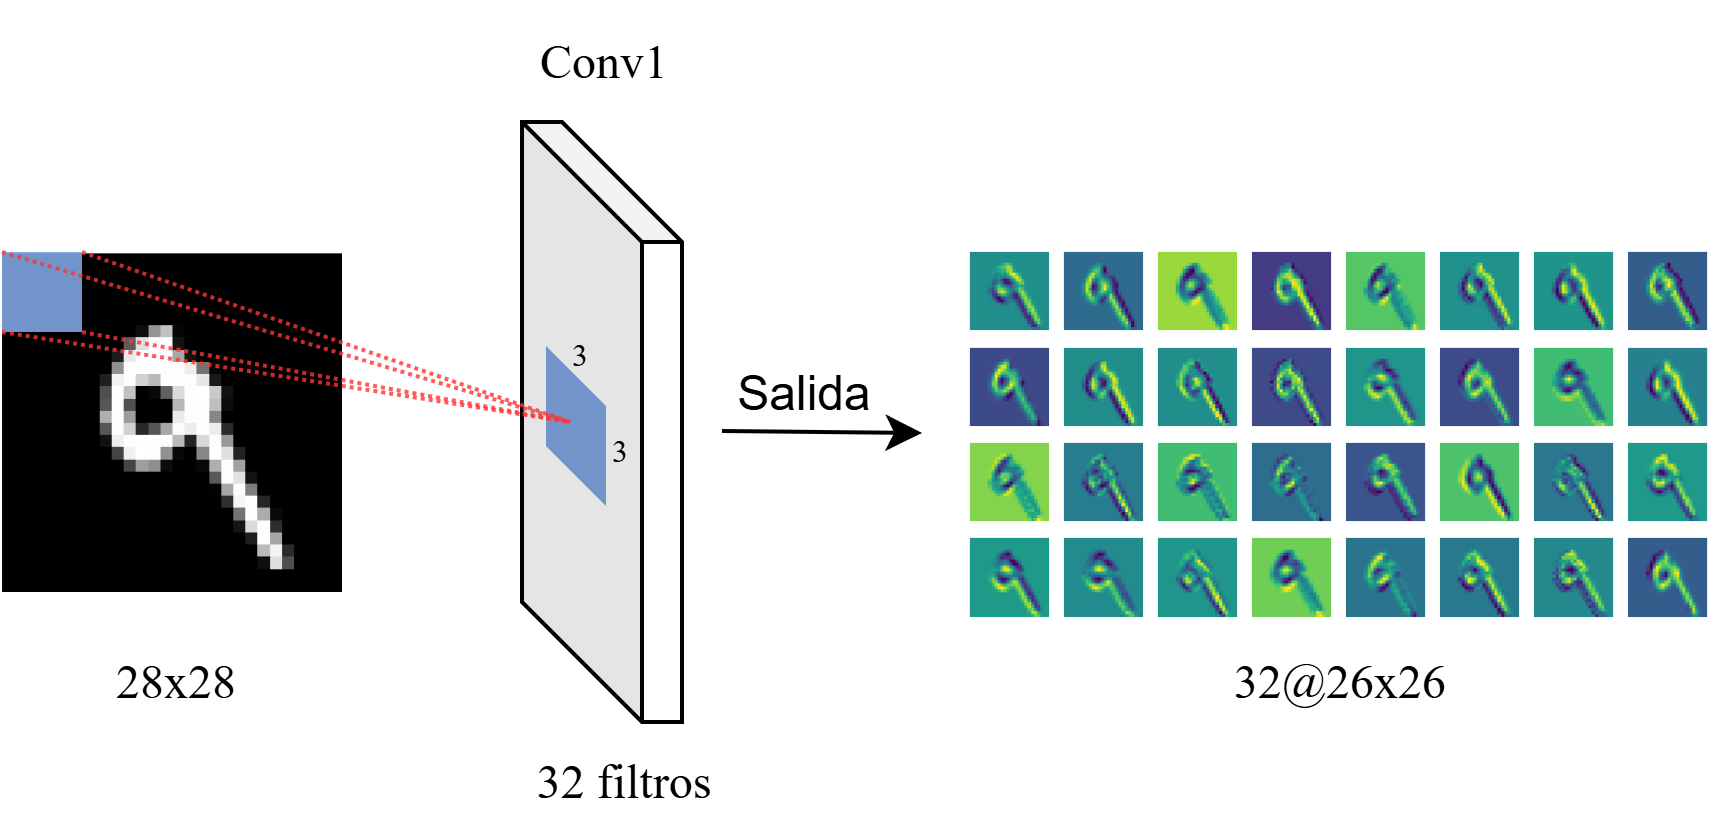
\includegraphics[width=1\linewidth]{figures/ejemplos/conv1_salidas.png}
	\caption{Salida de una capa convolucional con $32$ filtros de $3\times3$.}
	\label{fig:conv1_salidas}
\end{figure}


\paragraph{Capa de activación}

Generalmente, las operaciones matriciales que estamos realizando sobre las entradas pueden descomponerse como una combinación lineal de la forma $W_2(W_1x)=(W_2W_1)x$. Esto aporta un inconveniente muy grande, ya que la complejidad de nuestra arquitectura se simplificaría en una combinación lineal de las entradas con los parámetros de la red, provocando que nuestro modelo no sea capaz de aprender patrones más complejos. Para corregir esta laguna en nuestra arquitectura convolucional, introducimos una herramienta utilizada de igual forma en los modelos tradicionales: las funciones de activación. Concretamente, en este trabajo se utiliza la ya mencionada ReLU (\ref{sec:relu}), definida como $f(x) = \max(0, x)$. Donde, para $x > 0$, el comportamiento es lineal, mientras que para $x \le 0$, la salida es constante, consiguiendo de esta forma introducir no linealidad en el modelo \cite{dl_fundamentos__casas_roma_2020, dl__goodfellow_2016}.

\begin{figure}[h]
	\centering
	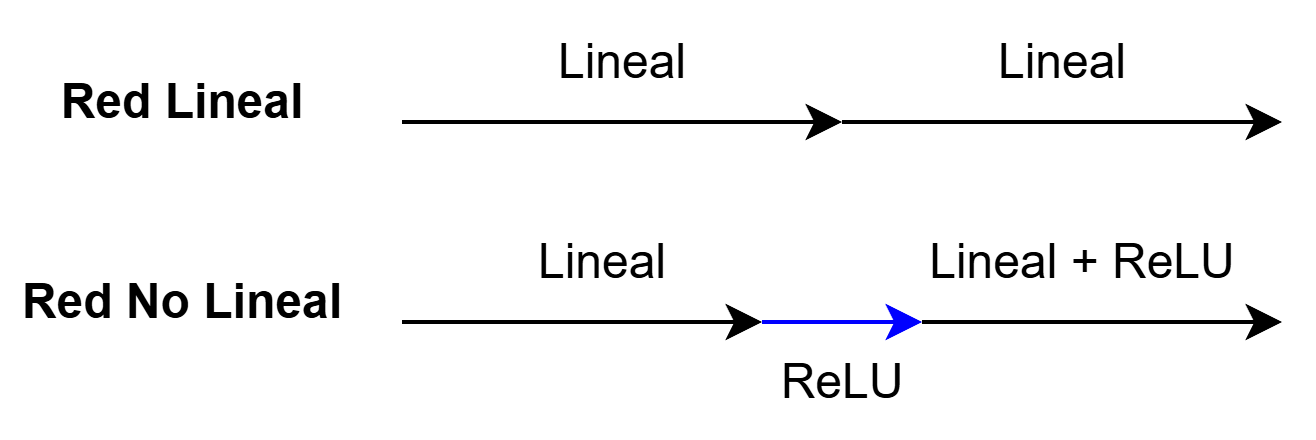
\includegraphics[width=0.6\linewidth]{figures/ejemplos/no_linealidad_relu.png}
	\caption{Comparación entre una red lineal y una con activación ReLU. La introducción de no linealidad permite modelar funciones más complejas.}
	\label{fig:relu_network}
\end{figure}


\paragraph{Capa de pooling}

Anteriormente, mencionamos que los modelos convolucionales tienen la capacidad de hacer una descomposición jerárquica de los datos de entrada. Las capas convolucionales, junto con las de activación, son las encargadas de extraer las características de nuestras imágenes. Sin embargo, nos falta un hilo conector muy importante para terminar de preparar esa información para las capas posteriores del modelo. Es aquí donde entran en juego las capas de pooling. La operación de pooling se refiere a una transformación cuya finalidad es reducir la dimensionalidad de la entrada. Para ello, normalmente se aplica una operación estadística el máximo, la media, o incluso la normalización L2, entre los valores seleccionados por una ventana de tamaño $n \times m$.

\begin{figure}[ht]
	\centering
	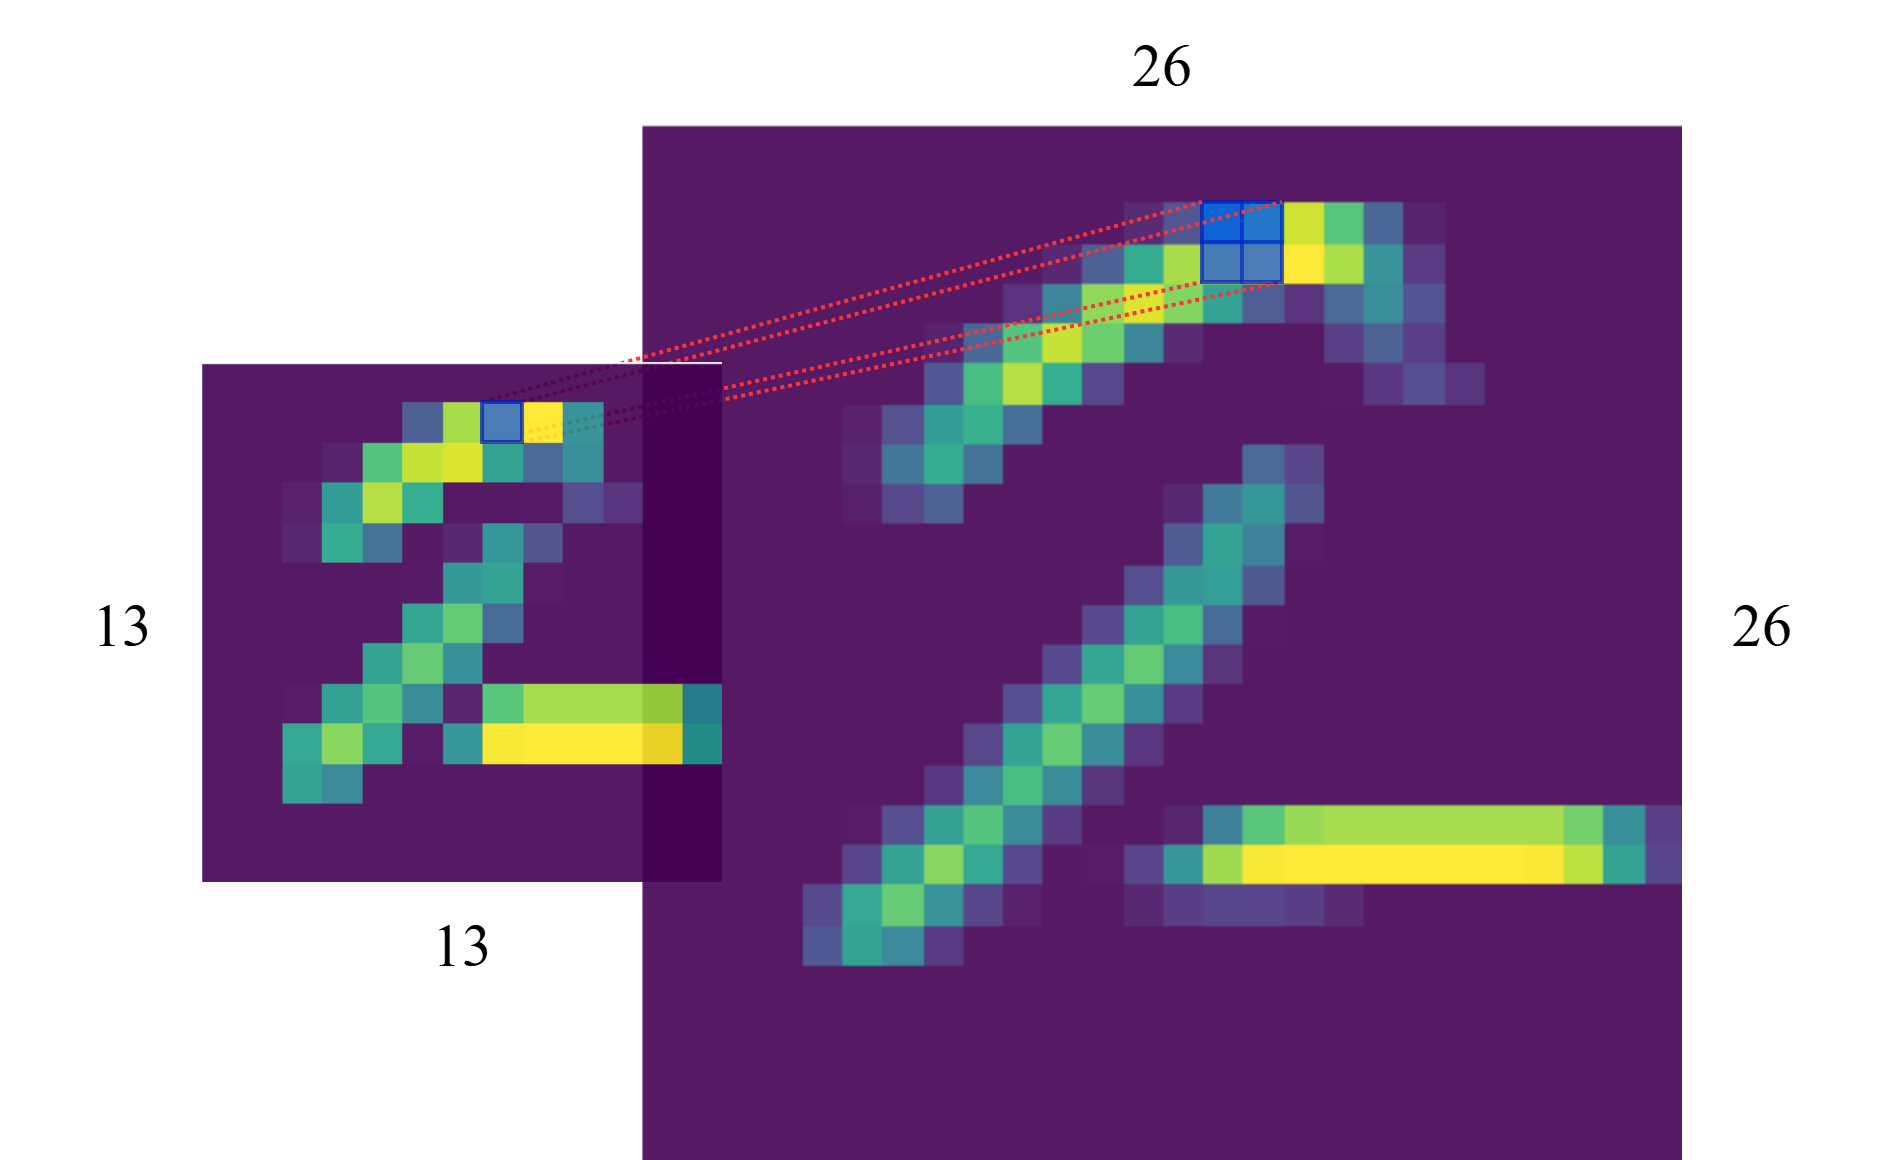
\includegraphics[width=0.8\linewidth]{figures/ejemplos/pooling_2d.png}
	\caption{Operación de Max Pooling con una ventana de $2\times2$.}
	\label{fig:pooling_2d}
\end{figure}

Además, las operaciones de pooling ayudan a que el modelo sea capaz de extraer y reconocer patrones sin importar pequeñas modificaciones en las entradas. Es decir, aplicando pooling introducimos invarianza ante traslaciones locales de las características, volviendo nuestra arquitectura más robusta. Algunos de los filtros de pooling más utilizados son el \textit{Max Pooling}, o el \textit{Avg Pooling} \cite{dl__goodfellow_2016}.

En la literatura y en las arquitecturas actuales, lo más común es encontrarnos la tríada de capas convolucional-relu-pooling, ya que esta configuración ayuda a dar robustez al modelo y permite construir estructuras más complejas y profundas sin que el rendimiento de la red se vea agravado.

\paragraph{Capa completamente conexa}

Llegamos a la parte final de nuestra arquitectura. Después de haber extraído todas las características aprovechando nuestros operadores espaciales, nuestra red introduce toda esa información en un conjunto de capas completamente conexas, similares a las de modelos tradicionales, donde se calcularán las relaciones entre los patrones extraídos y las clases sobre las que tenemos que predecir. Para ello, la salida de la última capa convolucional se suele aplanar para servir de entrada a la primera capa densa del modelo \cite{nn_dl__michael_nielsen_2015}.

Intuitivamente, podemos pensar en la arquitectura de una red convolucional como dos partes especializadas. La primera, que se encarga de extraer características útiles para identificar a las diferentes clases, lo cual tiene un coste computacional muy alto empleando arquitecturas tradicionales. Y la segunda, que se encarga de procesar esa información "masticada" previamente por el bloque convolucional, siendo capaz de inferir la pertenencia a cada clase.



\section{Funcionamiento Interno: Filtrado, Stride y Padding}\label{sec:funcionamiento_interno_cnn}

Como hemos ido viendo a lo largo de las secciones anteriores, las redes convolucionales se basan en la operación de convolución, donde un filtro se desplaza sobre la entrada y aplica una transformación con la que obtiene características concretas. Además, cada uno de estos filtros puede transformar dimensionalmente la entrada que reciben, reduciéndola, estirándola, etc. Por ello, a la hora de entrenar nuestros modelos, las dimensiones de los filtros, así como la forma en que los desplazamos por las entradas son hiperparámetros\footnote{Los hiperparámetros son parámetros de un modelo o del proceso de entrenamiento que \textbf{no se aprenden automáticamente} durante el entrenamiento, sino que los definimos nosotros previamente. Por ejemplo: el número de capas, la tasa de aprendizaje o el número de filtros a utilizar \cite{dl__goodfellow_2016}.} de configuración muy importantes, que pueden afectar directamente a la capacidad de la red para aprender y a la eficiencia computacional.

\paragraph{Dimensiones del filtro}

El tamaño de nuestros filtros es un factor clave dentro del aprendizaje. Filtros pequeños ($2\times2$ o $3\times3$) capturan detalles locales de la escena, algo así como si mirásemos desde un microscopio. Por otro lado, los filtros grandes ($7\times7$ o $11\times11$) permiten captar detalles más generales, con el inconveniente de requerir un mayor número de parámetros. Es decir, la dimensión que seleccionemos, no sólo va a determinar la forma en la que nuestro modelo aprenda, sino que va a afectar directamente en nuestro rendimiento computacional.

Además, desplazar un filtro de una determinada dimensión puede conllevar modificar la extensión de nuestra entrada en todos sus ejes. Es el caso de la figura \ref{fig:stride_avg_pooling} al pasar un filtro de tamaño $2\times2$ a nuestra entrada de $4\times4$, reducimos sus dimensiones a $3\times3$.

\paragraph{Stride}

Define el número de píxeles que avanza el filtro en cada paso. Con $\text{stride}=1$, el filtro se desplaza píxel a píxel, produciendo una salida de tamaño similar a la entrada. Con $\text{stride} \ge 2$, avanza dando saltos de $n$ píxeles tal que $n \ge 2$, reduciendo la dimensionalidad del resultado. A mayores valores, el stride provoca que la inferencia se haga muy rápido, con el inconveniente de que puede significar perder de información importante en las entradas.

\begin{figure}[h]
	\centering
	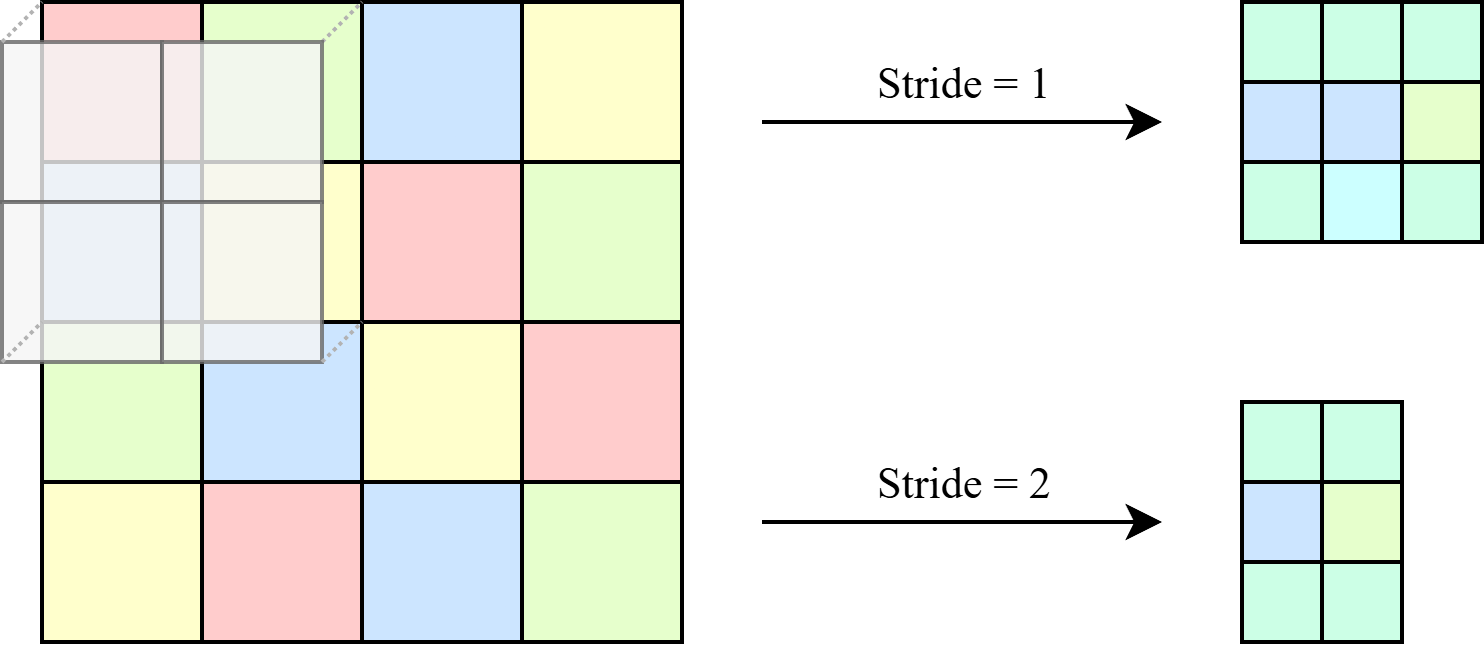
\includegraphics[width=0.65\linewidth]{figures/ejemplos/stride_avg_pooling.png}
	\caption{Ejemplo de average pooling con stride $= 1$ y stride $= 2$.}
	\label{fig:stride_avg_pooling}
\end{figure}

\paragraph{Padding}

En una convolución, al aplicar un kernel sobre una imagen, los píxeles situados en los bordes se "visitan" menos porque el filtro no puede extenderse más allá de los límites de la imagen. Este hiperparámetro nos permite configurar filas y columnas extra de relleno, normalmente a $0$, alrededor de la imagen para preservar la información de los bordes. Además, ajustando bien el padding podemos mantener el tamaño de entrada. Por ejemplo, una imagen de $4 \times 4$ con un filtro de $3 \times 3$ devuelve una imagen de $2 \times 2$. Con el padding adecuado, en este caso $\text{padding}=1$, puede mantenerse en $4 \times 4$. Es decir, el padding nos permite controlar el equilibrio entre reducir la dimensionalidad y preservar la información.

\begin{figure}[h]
	\centering
	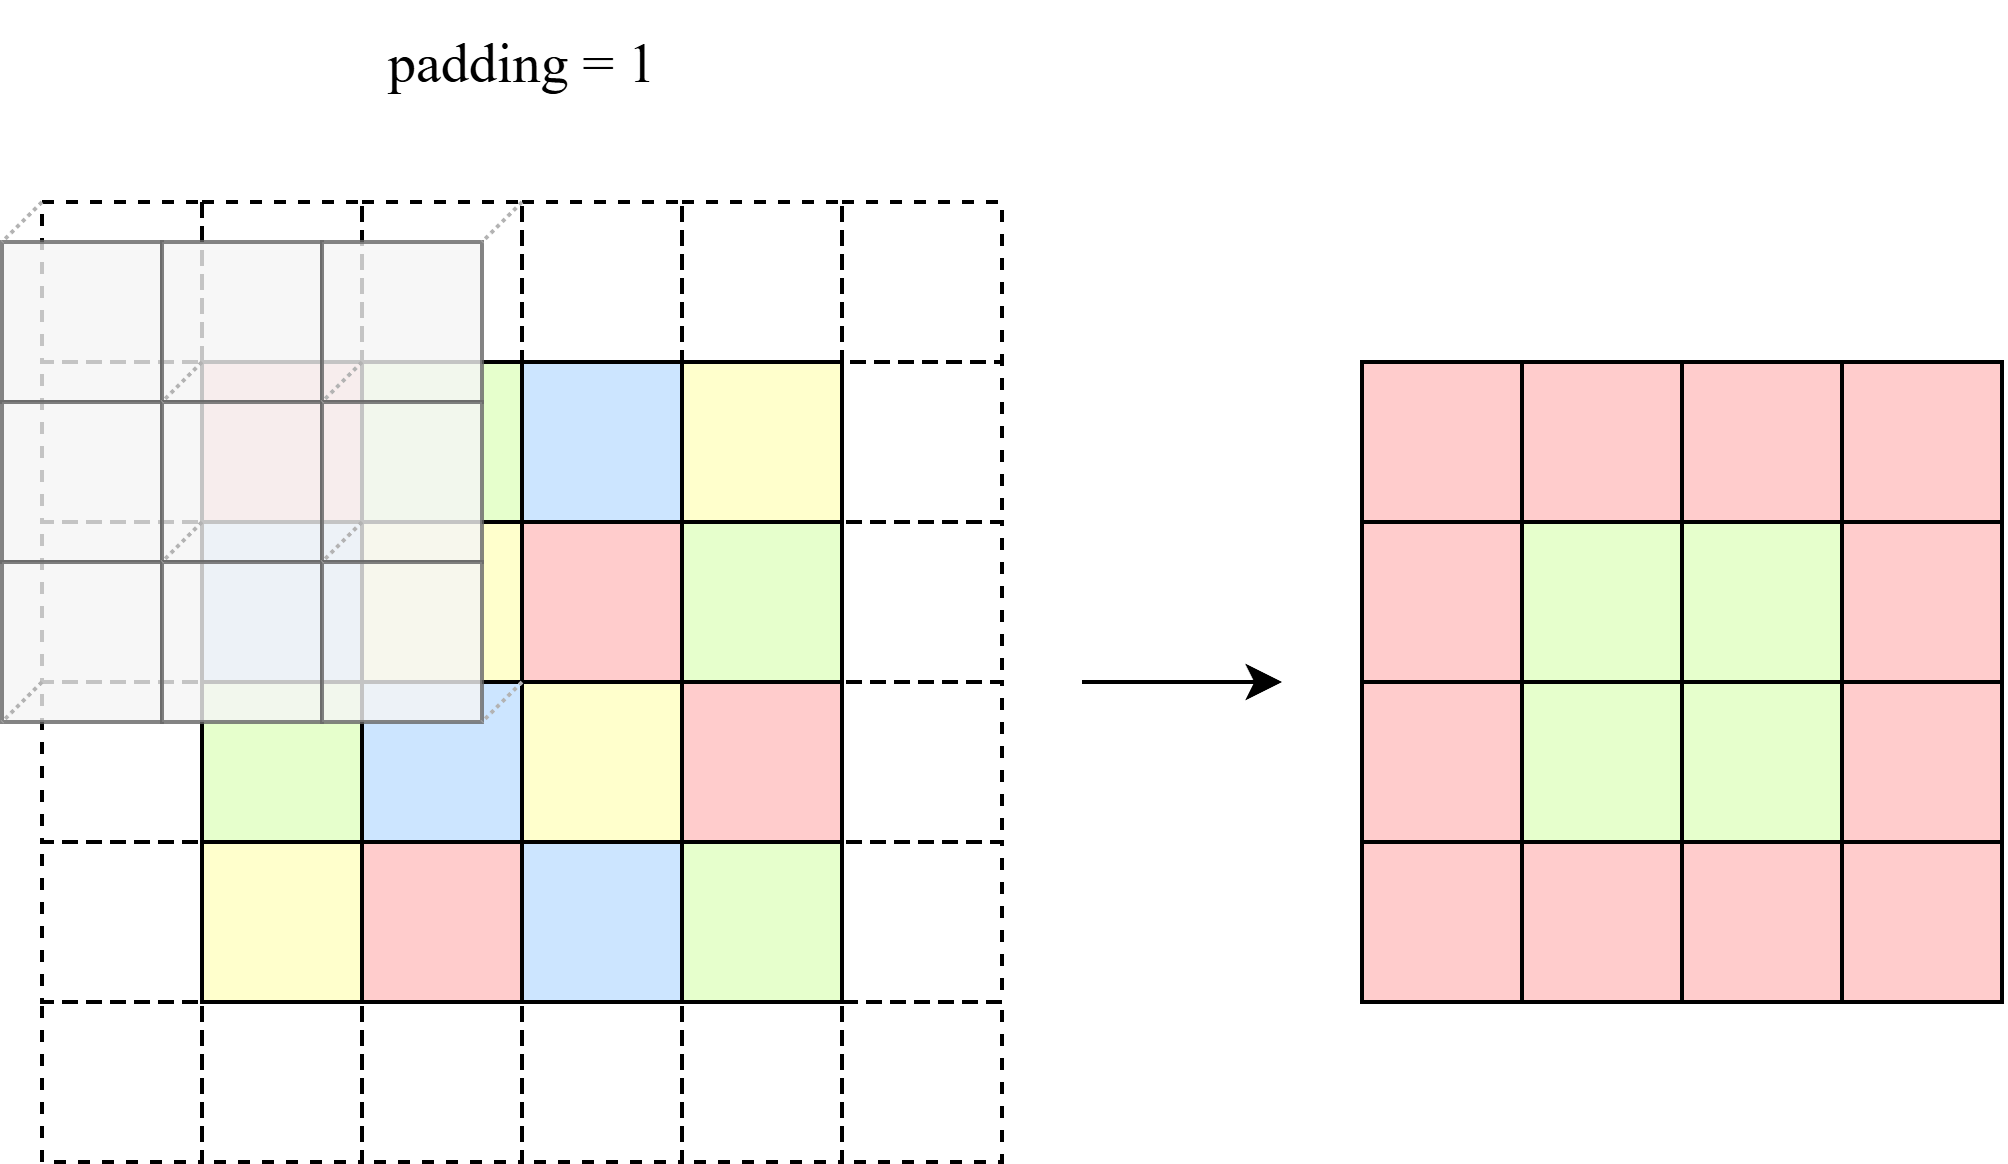
\includegraphics[width=0.8\linewidth]{figures/ejemplos/padding_avg_pooling.png}
	\caption{Ejemplo de average pooling con $\textbf{padding}=1$.}
	\label{fig:padding_avg_pooling}
\end{figure}

De esta forma, diseñar las capas convolucionales de nuestra red se convierte en un meticuloso trabajo artesanal para ajustar estos hiperparámetros de modo que la potencia del modelo y su eficiencia computacional estén equilibrados \cite{dl_python__chollet_2021, dl_fundamentos__casas_roma_2020, dl__goodfellow_2016}.



\section{Aprendizaje y Optimización de Filtros}\label{sec:ajuste_parametros_cnn}

El verdadero poder de las redes convolucionales reside en su capacidad de aprender de forma automática los filtros adecuados para extraer las características específicas que le permitan discernir adecuadamente entre las diferentes clases. Aquí entra en juego nuestro algoritmo de aprendizaje por antonomasia, la retropropagación. Al igual que los modelos tradicionales ajustan los pesos sus conexiones en base al error obtenido, los modelos convolucionales aprovechan estas iteraciones para afinar sus filtros.

\paragraph{Retropropagación en las capas convolucionales}

El aprendizaje de los filtros sigue el mismo principio que en modelos tradicionales: los pesos (en este caso, los valores de los kernels) se inicializan aleatoriamente y se ajustan iterativamente mediante el algoritmo de retropropagación del error (\ref{sec:retropropagacion}).
La retropropagación permite calcular el gradiente de la función de pérdida con respecto a cada parámetro de la red, propagando los errores desde la capa de salida hacia las capas anteriores. Este gradiente se usa para actualizar los pesos en la dirección que se minimiza la pérdida.

\paragraph{Optimización}

Para actualizar los parámetros, se utilizan algoritmos de optimización basados en el descenso del gradiente \ref{sec:descenso_gradiente}. El descenso de gradiente estocástico (SGD) es la técnica clásica, donde los parámetros se actualizan tras cada minibatch de datos.
En la práctica, se emplean variantes más sofisticadas como Adam, RMSProp o Momentum, que aceleran la convergencia y mejoran la estabilidad del entrenamiento \cite{dl_python__chollet_2021}.



\subsection{Visualización de activaciones}

{\color{red} AÑADIR IMÁGENES DE LAS ACTIVACIONES}

Una forma de comprender mejor cómo aprende nuestro modelo, y así, lograr un mejor ajuste de hiperparámetros o detectar posibles problemas en el entrenamiento, es mediante una técnica conocida como la visualización de activaciones. Consiste en inspeccionar los mapas de características que produce cada filtro en distintas capas de la red al procesar una imagen.
En las primeras capas suelen observarse activaciones asociadas a bordes y texturas simples, mientras que en capas más profundas aparecen representaciones cada vez más abstractas, como formas u objetos parciales \cite{dl_python__chollet_2021}.


